\documentclass[10pt,a4paper,final,oneside,openany,article,twocolumn]{memoir}
% [12pt, 11pt, landscape, titlepage, a4paper, draft, twoside, oneside, 
%  openleft, openright, openany]

%\chapterstyle{article}

%BASIC PACKAGES
\usepackage{eso-pic,fix-cm,ae,aecompl,ifthen}         
\usepackage[danish,english]{babel} % last language decides document language!
\usepackage[utf8x]{inputenc}          %text encoding
\usepackage{amsmath,amssymb, amsbsy}  % math
\usepackage{graphicx}
\usepackage[usenames,dvipsnames]{color}
\usepackage[british]{isodate} 
%\usepackage{morefloats}
\usepackage[style=alphabetic,natbib=true]{biblatex}
\usepackage{amsmath}
\usepackage[sc]{mathpazo}
\usepackage{MnSymbol}
\usepackage{booktabs} % nicer spacing between table rulers

\usepackage{fixltx2e} % To prevent the figures from being placed out-of-order with respect to their "non-starred" counterparts

%\bibliographystyle{apalike}
\bibliography{../bibliography}


\newsubfloat{figure}

%MISC. PACKAGES
%\usepackage{multicol}        % \begin{multicols}{2} \end{multicols}
%\usepackage{array}           % advanced tables
%\usepackage{multirow}        % advanced tables
%\usepackage{longtable}       % split tables over pages
%\usepackage{textcomp}        % symbols
%\usepackage{verbatim}        % monospace code environment
%\usepackage{pdflscape}       % \begin{landscape} \end{landscape}
%\usepackage{semantic}        % Good for proof trees and math ligatures
\usepackage[noend]{algorithmic}
\usepackage{algorithm}
\usepackage{microtype}        % AWESOME typography!
%\usepackage{colortbl}
%\usepackage{marvosym}
%Kan bruges som \fixme{blabla}. Vises sålænge tex doc er i draft.
\usepackage[draft]{fixme}


%FONT
\usepackage[T1]{fontenc}
\usepackage{palatino}              % font : garamond
\linespread{1.05}                  % Palatino needs more leading (space between lines)
%\usepackage[scaled]{beramono}
\renewcommand{\ttdefault}{cmtt}    % alternative monospace font
%\renewcommand{\rmdefault}{ugm}
%\usepackage{euler}                % weirdo math
%PAGE DIMENSIONS

%\usepackage[left=4.5cm, right=4.5cm, top=4.4cm, bottom=4.5cm]{geometry}


%HEADERS
\makepagestyle{myheadings}

%\makepsmarks{myheadings}{
%  \def\chaptermark##1{\markboth{%
%    \ifnum \value{secnumdepth} < -1
%      \if@mainmatter
%        \chaptername\ \thechapter\ --- %
%      \fi
%    \fi
%    ##1}{}}

%  \def\sectionmark##1{\markright{%
%    \ifnum \value{secnumdepth} < 0
%      \thesection. \ %
%    \fi
%    ##1}}
%}
%%\makeevenhead{myheadings}{\thechapter\hskip.3cm\vrule\hskip.3cm \leftmark}{}{}
%\makeoddhead{myheadings}{}{}{\leftmark\hskip.3cm\vrule\hskip.3cm\thechapter}
%%\makeoddhead{myheadings}{}{}{\rightmark\hskip.3cm\vrule\hskip.3cm\thesection}
%\makeevenfoot{myheadings}{}{\thepage}{}
%\makeoddfoot{myheadings}{}{\thepage}{}
%\pagestyle{myheadings}

% customize chapter pages

\makepagestyle{myheadingschapterpage}
  \makeevenfoot{myheadingschapterpage}{}{}{\thepage}
  \makeoddfoot{myheadingschapterpage}{}{}{\thepage}
\aliaspagestyle{chapter}{myheadingschapterpage}
\aliaspagestyle{title}{myheadingschapterpage}
\makeevenhead{myheadings}{}{\scshape \thetitle}{}
\makeoddhead{myheadings}{}{\footnotesize\scshape \thetitle}{}
\makeevenfoot{myheadings}{}{}{\thepage}
\makeoddfoot{myheadings}{}{}{\thepage}
\pagestyle{myheadings}



%PDF OUTPUT
\usepackage{hyperref}             % clickable url's in PDF-output
\hypersetup{
%    unicode=true,          % non-Latin characters in Acrobat’s bookmarks
%    pdftitle={My title},    % title
%    pdfauthor={Author},     % author
%    pdfsubject={Subject},   % subject of the document
%    pdfcreator={Creator},   % creator of the document
%    pdfproducer={Producer}, % producer of the document
%    pdfkeywords={keywords}, % list of keywords
%    pdfnewwindow=true,      % links in new window
    colorlinks=true,       % false: boxed links; true: colored links
    linkcolor=black,          % color of internal links
    citecolor=black,        % color of links to bibliography
    filecolor=black,      % color of file links
    urlcolor=black           % color of external links
}




%PRETTY COLORS
\usepackage{color}
\definecolor{blue}{rgb}{0,0,0.8}
\definecolor{green}{rgb}{0,0.5,0}
\definecolor{red}{rgb}{0.5,0,0}
\definecolor{grey}{rgb}{0.5,0.5,0.5}


%SECTION TITLES
\def\thefigure{\arabic{figure}}
%\def\thesection{\arabic{section}}
%\def\thesubsection{\thesection.\arabic{subsection}}
%\def\thesubsubsection{\alph{subsubsection}.}
% \alph \roman \arabin
\setcounter{tocdepth}{1}


% USER DEFINED COMMANDS AND ENVIRONMENTS
%\newcommand{\codevar}[1]{{\tt{\it #1}}}
%\newcommand{\genericleft}{\langle\hspace{-2.6pt}\vert}  % prints [[
%\newcommand{\genericright}{\vert\hspace{-2.6pt}\rangle} % prints ]]
%\newcommand{\generic}[1]{\genericleft #1 \genericright^{\varepsilon}}

%FIGURE CAPTIONS
%\usepackage[labelformat=empty]{subfig}
\usepackage{sidecap} % side captions: \begin{SCfigure}[2.7][ht] ...
\usepackage{caption}
\captionsetup{margin=0pt, font=small, labelfont=bf, format=hang}
\setlength{\abovecaptionskip}{0pt}
\setlength{\belowcaptionskip}{0pt}

%LINE SPACING
%\usepackage{setspace}
%EXAMPLE:
% \singlespacing, \onehalfspacing, \doublespacing, \setstretch{x}


%PROGRAM CODE WITH HIGLIGHTING AND SHAZZ!
%\usepackage{listings}



%DOCUMENT INFO
\title{\vspace{-3cm}
  Fitting an All-atom Protein Model to a $C_\alpha$-trace\\
}
\author{
	Martin Dybdal -- \texttt{dybber@dybber.dk}\\
	Anders Boesen Lindbo Larsen -- \texttt{abll@diku.dk} \\
	Esben Skaarup -- \texttt{sben@sben.dk}
}

%\datebritish
\date{16th July 2010}

\newcommand{\subimgwidth}{.48\textwidth}
\newcommand{\imgwidth}{.85\textwidth}
\renewcommand\v[1]{\boldsymbol{#1}}
\newcommand{\Ca}{C$_{\alpha}${}}
\newcommand{\rotateAround}[1]{\lcirclearrowright \hspace{-3mm}\colorbox{white}{}{} \hspace{-1.7mm} _{\scriptscriptstyle #1}}
\setcounter{secnumdepth}{1}
\setcounter{chapter}{0}
%\renewcommand\thesection{\arabic{section}}
\setsecheadstyle{\large\bfseries\raggedright}
\setsubsecheadstyle{\bfseries}

\twocoltocetc
\setlength{\absleftindent}{1.5cm}
\setlength{\absrightindent}{\absleftindent}
			
\begin{document}
\twocolumn[\maketitle
\begin{onecolabstract}
  Protein structure prediction is often simplified by using a model
  that only includes few of the atoms actually present in proteins. In
  particular, the algorithms group at our department only predicts a
  folding of the $C_\alpha$-trace, and are thus excluding most
  backbone atoms and all side-chain molecules.

  In this report we will investigate a strategy for predicting the
  native structure of proteins including all atoms (an all-atom
  model). Our method uses an already folded $C_\alpha$-trace as target.
  \vspace{0cm}
\end{onecolabstract}
]
\tableofcontents*

\newpage


\hspace{0.5cm}\includegraphics[width=0.4\textwidth]{figures/forside.png}

\listoffixmes

\newpage
\chapter{Introduction}
\label{chap:intro}
Proteins is the perhaps most important molecules of living
organisms. They perform a multitude of biological tasks and is found
in all lifeforms, from bacteria and unicellular organisms to
multicellular organisms such as animals. The chemical abilities and
biological functions of proteins is determined by their
three-dimensional structure. The ability to determine this structure
without performing costly experiments will have many applications in
medicine (e.g. drug design) and biotechnology. Protein structure
prediction and the related topic protein folding\footnote{The two
  research fields are distinguished by whether the actual folding
  process is simulated (protein folding) or a legal structure is
  sought without computing the intermediate steps (protein structure
  prediction).} are large and active research fields. It is still an
open problem.

\section{Protein structure}
The building blocks of proteins are amino acids\footnote{A detailed
  introduction to the structure of proteins is found in
  \cite{branden}}. There are twenty different amino acids which all
share a common structure. The type of amino acid is identified by an
attached molecule called the side-chain. A protein consists of one or
several unbranched chains (polymers) of amino acids. The order of
amino acids in such a chain is the primary structure of the protein.
The structure diagram in Figure \ref{fig:amino_connect} shows how a
sequence of amino acids are connected. The carbon atom connecting the
backbone with the side-chains is called the $C_\alpha$-atom. It is the
torsional angles around the two bonds connecting $C_\alpha$-atoms with
its neighbours ($N-C_\alpha$ and $C_\alpha-C'$), that contributes with
the highest variability to the determination of the protein structure
(see Section \ref{chap:protein_geometry}). Thus, when solving the
structure prediction problem it is common \fxwarning{cite} to cut down
the problem by using a model that describes the protein solely by its
$C_\alpha$-atoms. Such a sequence of $C_{\alpha}$ atoms is called a
$C_{\alpha}$-trace (see Figure \ref{fig:Calpha_backbone}). This is
also the representation used by the algorithms group at our department
and they have therefore requested a method for subsequently adding the
remaining atoms to their model.

In Section \ref{chap:protein_geometry} we will describe the geometry
of the protein backbone and its side-chains in detail.

%% Evt. Secondary structure: $\alpha$-helices, $\beta$-sheets
%% (+strands) and loops/turns.


\begin{figure}
  \centering
  \subbottom[]{
    \includegraphics[width=0.48\textwidth]{figures/Calpha_backbone}  
    \label{fig:Calpha_backbone}
  }
  \subbottom[]{
    \includegraphics[width=0.48\textwidth]{figures/amino_connect}  
    \label{fig:amino_connect}
  }
  \caption{(a) $C_{\alpha}$-trace. (b) All-atom protein backbone, with $R_1$, $R_2$ and $R_3$ representing side-chains}
\end{figure}

\section{Protein structure prediction}
The chemical stability of a protein molecule is determined by the
amount of free energy in its structure. It is hypothesized
(\textit{Anfinsens dogma} or the \textit{thermodynamic hypothesis},
\cite{anfinsen73, soundararajan2010}) that all proteins has a unique
stable conformation where the free energy is minimized. This
conformation is known as the native structure of the
protein. Determining it computationally is the problem of protein
structure prediction. Thus, protein structure prediction is an energy
minimization problem.

% Why simplifications are necessary to make the problem
% computationally feasible.

There are generally two approaches to protein structure prediction.
\textit{Comparative modelling} uses information from known template
proteins with similar amino acid sequences while performing the
prediction. Another approach, called \textit{ab initio} or
\textit{de novo}, starts ``from scratch'' in the sense that no
information from known structures are used, but instead the
physical/chemical interactions between atoms forms the basis. This
\textit{ab initio} strategy is the approach taken by the algorithms
group at our department.

\subsection{Evaluating predictions}
%http://cnx.org/content/m11608/latest/
To determine the quality of prediction algorithms it is common \fxwarning{cite}
to compare predicted structures of a test proteins with the actual
known structure of that protein. The known structure of such test
proteins are obtained by other means (e.g. X-ray crystallography).
Thus a comparison measure between protein conformations are
needed. The most widely used comparison measure is \textit{least root mean
  square deviation}, lRMSD. RMSD is based on the distances between
corresponding atoms in the two protein conformations under comparison.
If $\vec{A}$ and $\vec{B}$ are two different conformations of the same protein,
where $\vec{a}_i$ and $\vec{b}_i$ are the respective coordinates of atom $i$ in the two
structures, RMSD can be computed by:
\begin{equation}
  \label{eq:rmsd}
  D(\vec{A}, \vec{B}) = \sqrt{\frac{1}{n}\sum_{i=1}^n |\vec{a}_i - \vec{b}_i|^2}
\end{equation}
To compute lRMSD, the RMSD has to be minimized by rotation and
translation of the two conformations. That is, to compute lRMSD, an
\textit{optimal superpositioning} of the conformations is found and
RMSD is computed.


% Limitation: A realistic energy calculation will require an insight in biochemistry
% that is beyond the scope of this project.  Therefore, we limit
% ourselves to minimize the number of clashes as well as the deviation
% from the provided $C_\alpha$-trace.


\section{Our strategy}
As mentioned, the algorithms group at our department uses a model that
only includes the the $C_\alpha$-atoms. Our goal with this project is
to extend this model with the remaining atoms to get an all-atom
model.  This will also enable the algorithms group to participate in
the CASP experiment \cite{caspwebsite}.

The strategy we will pursue, is to use a given $C_\alpha$-trace
generated by their prediction algorithm as target when fitting a
protein model that contains all atoms. The fitting should be conducted,
such that it minimizes the number of clashes and at the same time
minimizes the deviation from the target $C_\alpha$-trace.

We consider our fitting problem as two somewhat separate problems.
First, the backbone must be fitted to the \Ca-trace, only minimizing
the deviation to the $C_{\alpha}$-trace.  Hereafter, the amino acid
side-chains are added to the backbone changing the backbone
conformation only if necessary.  In the following we have chosen to
consider these two tasks separately even though the residue handling
will cause changes in the backbone.

In Section \ref{chap:fitting_backbone}, we will describe the strategy we use to fit the all-atom backbone to the \Ca-trace ignoring the amino acid residues.
In Section \ref{chap:handling_sidechains}, we will explain how we add the side-chains to the all-atom backbone changing the backbone-conformation only if necessary.

%%% Local Variables: 
%%% mode: latex
%%% TeX-master: "rapport"
%%% End: 


\chapter{Protein geometry}
\label{chap:protein_geometry}
\begin{figure*}
  \centering
  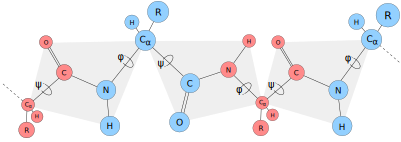
\includegraphics[width=0.75\textwidth]{figures/protein-torsion-angles}
  \label{fig:protein-torsion-angles}
  \caption{}
\end{figure*}

The representation of proteins shown in the structure diagram of
Figure \ref{fig:amino_connect} is suitable for determining the
chemical properties of the molecules, how atoms are arranged and the
bonding between atoms. However, to be able to do calculate on the
precise structure of the proteins we need a more precise
description. That is, we need to include bond lengths, bond angles and
torsional angles into the model.

\section{Backbone geometry}
Torsion angles, phi, psi, (omega)
Bond lengths
Bond angles

% As mentioned in our introduction, the largest variability of the
% protein structure is found in the \textit{torsional} angles between
% the individual $C_\alpha$-atoms \cite{lotan04}. These angles are
% termed $\phi$ and $\psi$ in the literature, Figure
% \ref{fig:protein-torsion-agnles} illustrates their definition.

\section{Side-chain geometry}
Rotamers (evt. calculating bond angles and bond lengths)


\chapter{Fitting the all-atom backbone}
\label{chap:fitting_backbone}
The first part of our fitting algorithm is to fit the protein backbone to the given \Ca-trace ignoring the side-chain conformations.

As input we are given a \Ca-trace target and a protein in form of an amino acid sequence.
Only the amino acid types are provided; no spatial structure information about the protein is given as this is left to the fitting algorithm to find.


\section{Limitations}
The adjustable parameters in a protein backbone structure consists of bond angles, dihedral angles and bond lengths.
As the dihedral angles are by far the most influencial parameters w.r.t the overall protein structure, we allow ourselves to perform the simplification of not considering bond lengths and bond angles.
More specifically, we will only consider the $\phi$ and $\psi$ angles and use a bacbone structure template for all other parameters.
Thus, the protein bacbone to be folded is a sequence of identical amino acid backbones that can only be modified by adjusting $\phi$ and $\psi$ for each amino acid.


\section{Inverse kinematics}
With the above limitations in place the backbone fitting problem can be regarded as a simple inverse kinematics (IK) problem.
IK is the process of determining angles of joints in a chain of rigid links in order to achieve a desired pose of the entire spatial structure.
In our case, the spatial structure consists of a series of links (atom bonds) connected by joints (atoms).
The desired pose is simply to make a \Ca-atom in the protein come as close as possible to its corresponding \Ca-trace target. \fxfatal{skal vi indsætte en simpel IK-illustration her?} 
As we have decided not to touch the joint angles (bond angles), the only adjustable angles in the kinematic chain are the dihedral angles around the atom bonds.

Several IK methods exist and have been utilized in protein structure prediction:
\cite{shenkin1987} describe a Jacobian solution that provide a linear approximation capable of handling lower limit constraints on interatomic distances between certain atoms.
The partial derivatives in the Jacobian matrix models the movement of the end of the kinematic chain relative to the angular changes.
To calculate the necessary changes in the available angles, the Jacobian is inverted.
According to \cite{canutescu2003} this inversion may be ill posed if the Jacobian is close to singular.


%inverse kinematics methods calculate the necessary changes in the available angles to minimize the distance between an object (called the \emph{end effector}) and a desired destination.



%We begin from one end of the amino acid sequence by placing the first two amino acids such that they match the beginning of the \Ca-trace target.


%$||N - C|| \rotateAround{180^\circ} \rotateAround{90^\circ} \rotateAround{v}$

\begin{figure}
  \centering
	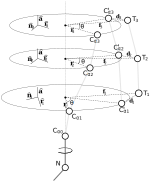
\includegraphics[width=0.75\columnwidth]{figures/ccd_angles}
	\label{fig:ccd_angles}
  \caption{}
\end{figure}



\chapter{Selecting side-chain conformations}
\label{chap:handling_sidechains}
In this section we will deal with the problem of placing side chains
on the protein and selecting side-chain conformations in a way that
minimizes the number of collisions.

As we mentioned in Section \ref{chap:protein_geometry}, statistical
analysis has shown that each type of amino acid side-chain has a small
set of common conformations \cite{dunbrack2002rotamer}. A side-chain
conformation is a configuration of its $\chi$ angles and is called a
\textit{rotamer}.

There has been developed several \textit{rotamer libraries}
\cite{dunbrack1997bayesian, lovell2000penultimate}, containing lists
of the common rotamers for each side-chain together with a probability
of each of those rotamer occuring in a protein. A comparison of some
(but not the most recent) rotamer libraries can be found in
\cite{dunbrack2002rotamer}. We have selected to use the rotamer
library made by Dunbrack et al. for the SCWRL side-chain
predictor\footnote{We use the latest release from 15th May 2002}.

\section{Our approach}
We have devised a simple algorithm for selecting side-chain rotamers
with the goal of minimizing the number of collisions between
atoms. Our first step is to apply the rotamer from the rotamer library
with highest probability to each amino in the protein. After this, we
go through each amino acid, this time trying to eliminate eventual
collisions. We use a breadth-first search through a tree that
represents the eventual collisions occuring for the different rotamers
of the amino acids. On Figure \ref{fig:rotamer-search-tree} we have
illustrated how our algorithm progresses, when trying to remove
collisions with a single amino acid. Each vertex represents an amino
acid and each edge represents a collision between the node and its
child. The names on the edges represents rotamers of the node
above. As an example, when rotamer \textit{k} is applied to amino acid
\textit{a}, \textit{a} collides with both \textit{c} and \textit{d}
(with their current rotamer, remember that we start by selecting the
most likely rotamer for all residues).

%% Hvornår kigger vi på rotameren som a startede ud med at have?

\begin{figure}
	\centering
	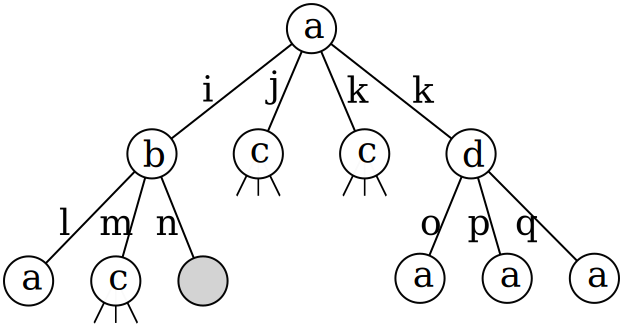
\includegraphics[width=.9\columnwidth]{figures/rotamersearch}
	\caption{The structure of our rotamer search space when eliminating
      collisions with the amino acid \textit{a}.}
    \label{fig:rotamer-search-tree}
\end{figure}

\section{Related Work}
The side-chain placement problem has been investigated by several
research groups, what we found most notably is the work done by
Dunbrack Labs on the SCWRL project \cite{canutescu2003graph,
  krivov2009improved}. To limit the search space, the algorithm of
SCWRL starts by removing rotamers with high self-energy from the set
of possible rotamers, as these are unlikely to be selected. Thus, they
need to use an energy function, which we have limited us from in our
project. Their next step is to resolve whether any collisions can be
transformed into disulfide bridges, which are bonds between two cysteine
amino acids from different places on protein but spatially near each
other.

% SCWRL: 
%  * Bruger energiberegning i valget af rotamerer
%  * Tjekker om par af cysteine amino syrer kan danne disulfid broer


% Todo: snak om SCWRL, der tilføjer side-chains på en fastlåst backbone.


%%% Local Variables: 
%%% mode: latex
%%% TeX-master: "rapport"
%%% End: 


\chapter{Evaluation and results}
Evaluering af metoden med kørsel på diverse kendte proteiner og
proteiner fra Rasmus

In our experience, a good value of $w$ is around 10 since a lookahead of 10 amino acids is sufficient to avoid good local conformation that lead to an unfavorable global conformation.
\begin{figure}
	\centering
	\hspace*{-3.5mm}\includegraphics[width=1.1\columnwidth]{figures/plot_rmsd}
	\caption{woop}
\end{figure}

\begin{figure}
	\centering
	\hspace*{-3.5mm}\includegraphics[width=1.1\columnwidth]{figures/plot_rmsd_convergence}
	\caption{woop}
\end{figure}

\begin{figure}
	\centering
	\hspace*{-3.5mm}\includegraphics[width=1.1\columnwidth]{figures/plot_collisions}
	\caption{woop}
\end{figure}


%TODO billede af foldet backbone med \Ca trace
%TODO ramachandran-plot




\chapter{Future Work}
The evaluation of our solution has revealed a couple of weaknesses that should be addressed. 

From the Ramachandran plot in Figure \ref{fig:eval_ramachandran_fitted} we see that the angles generated by the CCD method are not always realistic.
This could be improved by introducing Ramachandran probability maps.
A probability map is used by CCD to accept or reject proposed sets of $\phi$ and $\psi$ angles.
If a new set $\phi,\psi$ is proposed, the angles are chosen if they have higher probability than the current $\phi,\psi$.
If not, the angles are chosen with probability $p_{\text{new}}/p_{\text{old}}$. 
Probability maps for all amino acid types are available online, \cite{10.1371/journal.pcbi.1000763}, and should be straight forward to integrate.
Moreover, the use of probability maps has the benefit that the collision problem between the proline side-chain and the backbone is most likely to be eliminated as the illegal combination of angles is improbable. 

Another problem occurring when determining side-chain conformations is the inevitable collisions caused by an unfavorable backbone folding. 
To accommodate this situation, it could be relevant to investigate the possibility of using information from the side-chain structures to alter the backbone accordingly. 

So far, we have neglected the $\omega$ angle as $\omega$ angles different from 180$^\circ$ rarely occur. 
However, when it differs our backbone fitting method is penalized as the $\omega$ angle is locked.
If we should take $\omega$ into consideration, it would be inconvenient to include it in the CCD method like $\phi$ and $\psi$ as it is only supposed to be adjusted on rare occasions.
Instead, an $\omega$ test could be carried out on the entire backbone when it has been fitted to a low RMSD.
For a backbone with low RMSD, an incorrect $\omega$ angle will stand out.

Finally, we have mainly experimented with realistic proteins generated by X-ray crystallography. 
It would be interesting to do work with the \Ca-traces synthesized by the algorithms group, as these might introduce new difficulties.
\newpage

%\section{Experiment with Hydrogen atoms}
%How large is the variability of the hydrogen atoms in the backbone and
%side-chains? How hard would it be to add hydrogen atoms on to an
%otherwise full model of the protein? If the hydrogen atoms are easy to
%add later, we could post-pone the problem of adding them and thereby
%simplifying our model.


%%% Local Variables: 
%%% mode: latex
%%% TeX-master: "rapport"
%%% End: 


\chapter{Conclusion}

\defbibheading{bibliography}[\bibname]{
 \chapter{#1}
 \markboth{#1}{#1}}
\printbibliography

\end{document}

